% \subsection*{Arquitetura e Protocolos 5G}
A quinta geração de comunicações móveis celulares, o 5G, representa um avanço tecnológico sem precedentes, desenhado para revolucionar não apenas o setor de telecomunicações, mas a sociedade como um todo [1].

Essa geração foi projetada com o objetivo central de entregar taxas de dados substancialmente mais rápidas, conectividade mais confiável, cobertura aprimorada e latências rigorosamente baixas em comparação com as tecnologias predecessoras [2, 3].

As especificações de desempenho técnico e as diretrizes de avaliação da nova interface de rádio foram fundamentadas pelo padrão internacional conhecido como IMT-2020, concebido e monitorado pela União Internacional de Telecomunicações (ITU) [4, 5].

Para satisfazer a gama diversificada de requisitos estipulados no IMT-2020, o 3GPP (Third Generation Partnership Project) padronizou a tecnologia em sucessivos lançamentos, denominados de "Releases", definindo toda a arquitetura física e lógica fundamental do 5G [6, 7].

O escopo operacional do 5G foi idealizado em torno de três grandes cenários de uso ou áreas de serviço, os quais são vitais para a implantação das futuras infraestruturas digitais das cidades e da indústria [8].

O primeiro desses cenários, designado como Banda Larga Móvel Aprimorada (eMBB), visa a entrega de volumes extremos de dados móveis, suportando taxas de transferência de pico teóricas que alcançam 20 Gbps no downlink e 10 Gbps no uplink [9, 10].

O segundo cenário estratégico é o de Comunicações Massivas do Tipo Máquina (mMTC), que foi minuciosamente formulado para interconectar de forma eficiente o amplo ecossistema da Internet das Coisas (IoT), suportando inúmeros dispositivos interligados que requerem extrema economia de energia e baixo custo [9, 10].

O terceiro pilar é configurado pelas Comunicações Ultra-Confiáveis e de Baixa Latência (URLLC), um arranjo vital para aplicações de controle robótico, fábricas inteligentes e processos que demandam taxas de erro na casa de $10^{-5}$ e atrasos logísticos restritos a frações de milissegundos [10, 11].

Para dar sustentação tecnológica a tamanhas exigências, a arquitetura do ecossistema 5G foi subdividida em dois grandes blocos: a Nova Rede de Acesso de Rádio (NG-RAN) e o Core de Próxima Geração (5GC) [6, 12].

\begin{figure}[ht!]
\centering
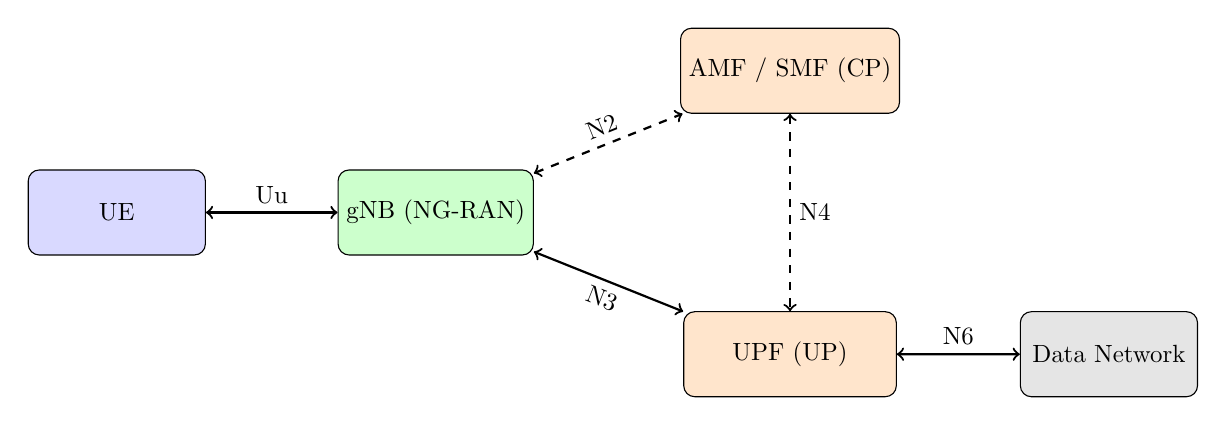
\begin{tikzpicture}[node distance=2cm, auto, scale=0.9, transform shape]
  % Nodes
  \node[draw, rectangle, rounded corners, fill=blue!15, minimum width=2.5cm, minimum height=1.2cm] (ue) {UE};
  \node[draw, rectangle, rounded corners, fill=green!20, minimum width=2.5cm, minimum height=1.2cm, right of=ue, node distance=4.5cm] (gnb) {gNB (NG-RAN)};
  \node[draw, rectangle, rounded corners, fill=orange!20, minimum width=3cm, minimum height=1.2cm, right of=gnb, node distance=5cm, yshift=2cm] (amf) {AMF / SMF (CP)};
  \node[draw, rectangle, rounded corners, fill=orange!20, minimum width=3cm, minimum height=1.2cm, right of=gnb, node distance=5cm, yshift=-2cm] (upf) {UPF (UP)};
  \node[draw, rectangle, rounded corners, fill=gray!20, minimum width=2.5cm, minimum height=1.2cm, right of=upf, node distance=4.5cm] (dn) {Data Network};

  % Edges
  \draw[<->, thick] (ue) -- node[above] {Uu} (gnb);
  \draw[<->, thick, dashed] (gnb) -- node[above, sloped] {N2} (amf);
  \draw[<->, thick] (gnb) -- node[below, sloped] {N3} (upf);
  \draw[<->, thick, dashed] (amf) -- node[right] {N4} (upf);
  \draw[<->, thick] (upf) -- node[above] {N6} (dn);
\end{tikzpicture}
\Caption{\label{fig:arquitetura_5g_short} Arquitetura Simplificada da Rede 5G (Plano de Controle e Usuário).}
\Fonte{Elaborado pelo autor.}
\end{figure}

O núcleo da rede, o 5GC, implementa o modelo de Arquitetura Baseada em Serviços (SBA), uma abordagem modernizada em que diversas funções de rede comunicam-se através de requisições de serviço em interfaces bem padronizadas [13, 14].

Esse núcleo avança significativamente em relação aos modelos prévios através da efetiva separação metodológica e estrutural do Plano de Controle e do Plano de Usuário (CUPS) [15, 16].

Impulsionado pelas capacidades do 5GC, surge o conceito inovador de Fatiamento de Rede (Network Slicing), em que a infraestrutura física de telecomunicações é dividida em incontáveis redes lógicas isoladas atuando em paralelo [17, 18].

Valendo-se do Fatiamento de Rede, cada rede virtual individual (slice) pode ser parametrizada para oferecer atributos únicos em termos de largura de banda, latência, mobilidade e segurança, enquadrando-se perfeitamente nos propósitos do cliente e na diversidade dos serviços digitais [18, 19].

\begin{figure}[ht!]
\centering
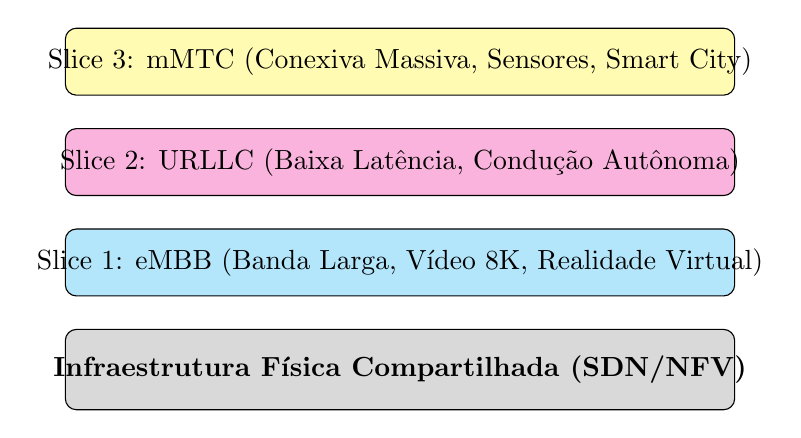
\begin{tikzpicture}[scale=0.85]
  % Infraestrutura física
  \draw[fill=gray!30, rounded corners] (0,0) rectangle (10, 1.2) node[midway, font=\bfseries] {Infraestrutura Física Compartilhada (SDN/NFV)};
  % Fatias (Slices)
  \draw[fill=cyan!30, rounded corners] (0,1.7) rectangle (10, 2.7) node[midway] {Slice 1: eMBB (Banda Larga, Vídeo 8K, Realidade Virtual)};
  \draw[fill=magenta!30, rounded corners] (0,3.2) rectangle (10, 4.2) node[midway] {Slice 2: URLLC (Baixa Latência, Condução Autônoma)};
  \draw[fill=yellow!30, rounded corners] (0,4.7) rectangle (10, 5.7) node[midway] {Slice 3: mMTC (Conexiva Massiva, Sensores, Smart City)};
\end{tikzpicture}
\Caption{\label{fig:slicing_short} Conceito de Fatiamento de Rede (Network Slicing) baseado em NFV/SDN.}
\Fonte{Elaborado pelo autor.}
\end{figure}

Essa grande flexibilidade operacional da rede e do núcleo é primariamente garantida pelas abordagens fundamentais em Redes Definidas por Software (SDN) e Virtualização de Funções de Rede (NFV) [20, 21].

A tecnologia NFV tem o papel revolucionário de abstrair as capacidades de computação e armazenamento da rede, implementando-as em software de forma ágil dentro de máquinas virtuais comerciais, dispensando a necessidade de grandes hardwares físicos proprietários [20, 22].

Em consonância, a diretriz do SDN isola a camada de dados da camada de decisões nos roteadores corporativos, consolidando de maneira eficiente as rotas a partir de um controlador unificado programável em servidor central [17, 20].

Ainda para viabilizar as baixas latências ditadas pelo URLLC, as funções e conteúdos de aplicações foram deslocados das nuvens centrais tradicionais para as extremidades locais, formando a chamada Computação de Borda de Múltiplo Acesso (MEC) [20, 23].

O emprego do MEC e a distribuição regional do elemento de núcleo UPF minimizam a dependência das onerosas ligações de longas distâncias, diminuindo o congestionamento nos datacenters centrais e melhorando a qualidade das transferências e experiências multimídia interativas [23, 24].

Quanto à infraestrutura na borda sem fio, a estação rádio base evoluiu drasticamente em relação aos antigos "eNodeB" do LTE 4G, passando a ser formalmente denominada "Next-generation Node B" ou gNodeB (gNB) [17, 25].

Esses complexos equipamentos gNBs foram desenvolvidos permitindo operações baseadas na separação rigorosa entre suas funções base: a Unidade Central (CU), responsável por processos de maior nível, e as Unidades Distribuídas (DU), localizadas mais perto da antena [26, 27].

Dada a amplitude das mudanças exigidas pela quinta geração, as operadoras elaboraram passos migratórios estratégicos, inicialmente focados na implantação baseada no modelo Não-Autônomo (NSA) [25, 28].

O modelo Não-Autônomo (NSA) ancora-se inicialmente sobre o núcleo consolidado de pacotes (EPC) do 4G, agregando portadoras e fornecendo conectividade dupla em que a torre 4G LTE atua como controladora primária enquanto a antena gNB 5G reforça vigorosamente o fluxo dos dados [25, 29].

Para finalizar a modernização, as redes se deslocam rumo ao 5G Autônomo (SA) definitivo, cenário chamado de Opção 2, em que a estação gNB se acopla livremente ao núcleo 5GC puro, concretizando funcionalidades de ponta a ponta sem qualquer arranjo residual do 4G LTE [28, 30].

Todas essas conexões via rádio com o usuário final operam utilizando uma arquitetura avançada de interface aérea global, devidamente conhecida por 5G New Radio (NR) [9, 31].

Na padronização do 5G NR, o espectro utilizável da rádio frequência sofreu uma dramática elevação das larguras de banda, dividindo as operações nos denominados Frequência Range 1 (FR1) e Frequência Range 2 (FR2) [32, 33].

O intervalo de rádio FR1 incorpora tipicamente o espectro da faixa sub-6 GHz, englobando canais em faixas que se estendem aos 7.125 GHz, o que possibilita um balanço crucial entre penetração em interiores e uma boa capacidade [34, 35].

Por outro lado, o verdadeiro salto para a massificação cibernética multicanal provém das ondas do intervalo FR2, cujas frequências, conhecidas como ondas milimétricas (mmWave), flutuam nas larguras extensas entre 24.25 GHz a 71 GHz [33, 35].

Inerente às leis físicas de transmissão nas extremas bandas milimétricas, a atenuação natural atmosférica reduz criticamente o raio geográfico alcançável das células instaladas nas torres urbanas [32, 36].

Para contornar as robustas dificuldades inerentes às altas perdas propagativas do FR2, introduziu-se obrigatoriamente a expansão dos sistemas de transmissão, implementando antenas Massivas do tipo Múltiplas Entradas e Múltiplas Saídas (Massive MIMO) [37, 38].

As estruturas compostas de Massive MIMO concentram densidades que superam dezenas de minúsculos componentes de antenas transmissoras empacotadas em um único painel [36, 39].

Valendo-se das centenas de elementos nestes painéis, a rede aplica complexos desvios de fase em tempo real para sintetizar sinais focais, num método essencial e revolucionário conceituado fisicamente como conformação de feixes ("Beamforming") [36, 40].

O Beamforming ativo dirige rigorosamente os focos das radiações milimétricas, anulando desperdícios de potência em rotas inúteis e entregando conexões muito mais eficientes ao usuário pontual e em movimento dinâmico [36, 39].

O emparelhamento do Massive MIMO permite a modulação de comunicação com múltiplos utilizadores paralelos sobre o mesmo elemento de tempo e frequência, estratégia tática estabelecida na arquitetura através do Multi-User MIMO (MU-MIMO) [37, 38].

Referente ao roteamento e espalhamento da forma de onda nos feixes, o downlink do 5G NR é fundado em bases de Multiplexação por Divisão de Frequências Ortogonais (OFDMA) para alocar os usuários nas subportadoras simultaneamente [41, 42].

Uma alteração proeminente do 5G sob a camada do OFDMA convencional é a incorporação nativa de "Numerologias", permitindo alterar geometricamente a lacuna das subportadoras em múltiplos flexíveis de 15, 30, 60 e até 120 kHz [43, 44].

Quanto maior for o espaçamento entre as referidas subportadoras do espectro OFDMA, exponencialmente mais curto o pacote ou o símbolo de duração de tempo propagado trafegará na infraestrutura aérea do ambiente radiante [45, 46].

Essa maleabilidade estrutural viabiliza os drásticos requisitos previstos pelo escopo URLLC para as aplicações sensíveis ao tempo (como na direção assistida e na telemetria rodoviária severa) que falhariam em transmissões síncronas compridas e inflexíveis [10, 45].

Em prol de garantir altíssima confiabilidade e correções de erros nessas altas taxas, o 5G NR padronizou avançados algoritmos físicos, descartando antigas formulações em favor de esquemas potentes baseados nos códigos de Paridade de Baixa Densidade, como as matrizes LDPC [47].

Combinando-se com os módulos FEC (Forward Error Correction) e LDPC, atua em paralelo o reenvio híbrido flexível de dados espaciais com confirmações automáticas HARQ (Hybrid Automatic Repeat Request) na detecção e recomposição dos sub-canais ofendidos no percurso [48].

\begin{figure}[ht!]
\centering
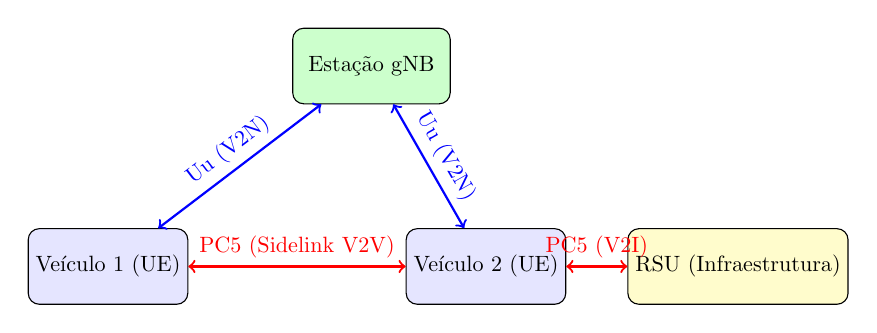
\begin{tikzpicture}[node distance=2.5cm, auto, scale=0.8, transform shape]
  % Nodes
  \node[draw, rectangle, rounded corners, fill=blue!10, minimum width=2.5cm, minimum height=1.2cm] (car1) {Veículo 1 (UE)};
  \node[draw, rectangle, rounded corners, fill=blue!10, minimum width=2.5cm, minimum height=1.2cm, right of=car1, node distance=6cm] (car2) {Veículo 2 (UE)};
  \node[draw, rectangle, rounded corners, fill=green!20, minimum width=2.5cm, minimum height=1.2cm, above right of=car1, node distance=4.5cm, xshift=1cm] (gnb) {Estação gNB};
  \node[draw, rectangle, rounded corners, fill=yellow!20, minimum width=2.5cm, minimum height=1.2cm, right of=car2, node distance=4cm] (rsu) {RSU (Infraestrutura)};

  % Edges
  \draw[<->, thick, red] (car1) -- node[above] {PC5 (Sidelink V2V)} (car2);
  \draw[<->, thick, blue] (car1) -- node[above, sloped] {Uu (V2N)} (gnb);
  \draw[<->, thick, blue] (car2) -- node[above, sloped] {Uu (V2N)} (gnb);
  \draw[<->, thick, red] (car2) -- node[above] {PC5 (V2I)} (rsu);
\end{tikzpicture}
\Caption{\label{fig:cv2x_short} Conceito 5G C-V2X abrangendo comunicações Uu (Celular) e PC5 (Sidelink direto).}
\Fonte{Elaborado pelo autor.}
\end{figure}

Desfrutando inteiramente dessa nova realidade construída com baixas latências de borda, surgem as aplicações da arquitetura C-V2X (Cellular Vehicle-to-Everything), engenhadas especificamente para orquestrar o trânsito moderno inteligente [3, 49].

As premissas baseadas em V2X no 5G impulsionam a permuta instantânea de posições geográficas entre veículos em alta velocidade, assim como entre redes veiculares cruzando sinalizações semafóricas dotadas de sensores independentes da malha civil [49, 50].

O avanço na maturação do padrão do 5G NR nas gerações pós-Release 16 impulsionou não apenas rastreamentos de frota, mas as exigentes tecnologias de "platooning" veicular avançado de automação veicular compartilhada sem intervenções do controle rodoviário humano [50, 51].

Dentro dos blocos lógicos desse segmento automotivo formidável, a pedra fundamental reside na estipulação rádio referenciada por Interface PC5, amplamente batizada na indústria pelas alcunhas de "Sidelink" [50, 52].

A capacidade "Sidelink" do 5G engendra autênticas comunicações radiais ponto a ponto orientadas de dispositivos para dispositivos (D2D) sem depender da coordenação em nuvens ou em trânsitos centrais via gNB para que os pacotes troquem de rotas cruciais [49, 50].

Ao harmonizar formidavelmente a capacidade multimegabit do feixe mmWave, o isolamento lógico das fatias NFV e as topologias diretas distribuídas em Sidelink e MEC, a quinta geração sela a base imutável para consolidar o avanço sem limites das sociedades veiculares urbanas nos anos seguintes [10, 51, 53].

Este capítulo aborda os princípios do processamento digital de sinais na interface aérea do 5G. Existem três tópicos principais. O primeiro abrange as técnicas subjacentes para transmissão e recepção que o 5G herdou dos sistemas 2G e 3G, como por exemplo, modulação, demodulação e estimativa de canal. O segundo abrange a multiplexação por divisão de frequências ortogonais (\gls{OFDMA}), uma técnica herdada do LTE através da qual a estação base pode se comunicar com diferentes dispositivos móveis simultaneamente. O terceiro abrange o gerenciamento de erros no fluxo de dados recebido por meio de correção antecipada de erro e retransmissão. Também serão discutidos uma série de problemas inerentes às elevadas frequências de rádio e que são especialmente relevantes ao 5G.

Este capítulo contém um amparo matemático maior que a maioria dos outros materiais, no entanto, foi mantido deliberadamente leve com o objetivo de tornar o estudo acessível para aqueles sem um denso embasamento em matemática avançada. A Bibliografia reúne referências chave para leitura complementar, tanto para o material explícito neste capítulo como para a matemática subjacente.

\subsection{Modulação e Demodulação}

\subsubsection{Sinal da Portadora}
Em um sistema de comunicação sem fio, a onda de rádio (vista no Capítulo 4) atua como um sinal de portadora. Matematicamente, nós podemos expressar o sinal da portadora através da seguinte função periódica:

\section{Arquitetura e Modelagem \texorpdfstring{\gls{5G}}{5G} \texorpdfstring{\gls{V2I}}{\gls{V2I}} e \texorpdfstring{\gls{C-V2X}}{C-\gls{V2X}}}
\label{sec:comunicacao-5g-e-sidelink}

A quinta geração de comunicações móveis celulares, o \gls{5G}, representou um avanço tecnológico disruptivo, projetado para revolucionar não apenas o setor de telecomunicações, mas também a sociedade como um todo~\cite{stallings2021}. Suas especificações foram fundamentadas pelo padrão internacional IMT-2020, sob avaliação e monitoramento da \gls{ITU}~\cite{itu2015m2083, itu2017m2410, itu2021m2150}, e formalizadas pelo \gls{3GPP} em sucessivos \textit{Releases}~\cite{asplund2025, cox2025}.

O \gls{5G} foi idealizado para operar em três grandes cenários de uso. O primeiro, \gls{eMBB}, atende serviços que exigem altas taxas de transferência de dados, suportando picos de até 20~Gbps no \textit{downlink}~\cite{stallings2021}. O segundo, \gls{mMTC}, foi formulado para interconectar eficientemente o ecossistema da \gls{IoT}, suportando um grande número de dispositivos com baixo consumo energético~\cite{morais2025, raghavan2025}. O terceiro, \gls{URLLC}, é essencial para aplicações que demandam atrasos na casa de frações de milissegundos e taxas de erro de $10^{-5}$, como controle robótico e \gls{ITS}, incluindo casos de uso avançados como o \textit{platooning}\footnote{Refere-se à aplicação de \gls{ITS} que vincula eletronicamente dois ou mais veículos para que trafeguem de forma coordenada, mantendo uma distância mínima e constante entre si.} e a direção autônoma de Nível 4 e 5~\cite{sae2021j3016, raghavan2025, sheikh2026}.

Para suportar tais exigências, a arquitetura do \gls{5G} foi subdividida em dois grandes blocos: (i) a \gls{NG-RAN}, responsável pelo acesso de rádio, e (ii) o \gls{5GC}, que implementa o núcleo da rede por meio do modelo de \gls{SBA}~\cite{stallings2021}, conforme ilustrado na Figura~\ref{fig:arquitetura_5g_macro}. No núcleo, as \gls{AMF} e \gls{SMF} gerenciam mobilidade, sessões e sinalização, enquanto a \gls{UPF} é responsável pelo roteamento efetivo dos pacotes de dados.

\begin{figure}[ht!]
\centering
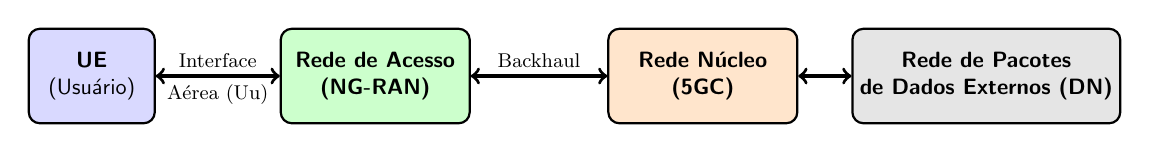
\begin{tikzpicture}[auto, thick, scale=0.8, transform shape, font=\sffamily]
  % Nodes
  \node[draw, rectangle, rounded corners, fill=blue!15, minimum width=2cm, minimum height=1.5cm, align=center] (ue) {\textbf{UE}\\(Usuário)};
  \node[draw, rectangle, rounded corners, fill=green!20, minimum width=3cm, minimum height=1.5cm, align=center, right of=ue, node distance=4.5cm] (ran) {\textbf{Rede de Acesso}\\\textbf{(NG-RAN)}};
  \node[draw, rectangle, rounded corners, fill=orange!20, minimum width=3cm, minimum height=1.5cm, align=center, right of=ran, node distance=5.2cm] (core) {\textbf{Rede Núcleo}\\\textbf{(5GC)}};
  \node[draw, rectangle, rounded corners, fill=gray!20, minimum width=2.5cm, minimum height=1.5cm, align=center, right of=core, node distance=4.5cm] (dn) {\textbf{Rede de Pacotes}\\\textbf{de Dados Externos (DN)}};

  % Edges
  \draw[<->, very thick] (ue) -- node[above, font=\small] {Interface} node[below, font=\small] {Aérea (Uu)} (ran);
  \draw[<->, very thick] (ran) -- node[above, font=\small] {Backhaul} (core);
  \draw[<->, very thick] (core) -- (dn);
\end{tikzpicture}
\Caption{\label{fig:arquitetura_5g_macro} Modelo de sistema básico \gls{3GPP} evidenciando os dois grandes blocos operacionais do \gls{5G}.}
\Fonte{Baseado no modelo de sistema \gls{3GPP}~\cite{fowdur2025}.}
\end{figure}

Para garantir baixas latências, foi necessário distribuir as funções de processamento e armazenamento da nuvem para dispositivos mais próximos do cliente do serviço. Na prática, isso significou que as aplicações não precisariam mais enviar seus dados para \textit{datacenters} distantes, evitando latências elevadas. Essa solução foi materializada com a integração do \gls{MEC} à rede móvel \gls{5G}, onde a \gls{UPF} é distribuída localmente para rotear os dados diretamente aos servidores periféricos, possibilitando a resposta em tempo real. A Figura~\ref{fig:arquitetura_mec_5g} ilustra a arquitetura do \gls{5GC} com a integração do \gls{MEC}.

\begin{figure}[ht!]
\centering
\begin{tikzpicture}[auto, thick, scale=0.85, transform shape, font=\sffamily]
  % Nodes Padrão
  \node[draw, rectangle, rounded corners, fill=blue!15, minimum width=2cm, minimum height=1.2cm] (ue) {UE};
  \node[draw, rectangle, rounded corners, fill=green!20, minimum width=2.5cm, minimum height=1.2cm, right=1.5cm of ue] (gnb) {NG-RAN};

  % Borda (Edge / MEC)
  \node[draw, rectangle, rounded corners, fill=orange!20, minimum width=2.5cm, minimum height=1.2cm, align=center, below=2cm of gnb] (upfl) {UPF\\ (Local)};

  % Core Central (5GC)
  \node[draw, rectangle, rounded corners, fill=orange!20, minimum width=2.5cm, minimum height=1.2cm, align=center, right=4cm of gnb, yshift=1.2cm] (amf) {AMF / SMF\\ (Controle)};
  \node[draw, rectangle, rounded corners, fill=orange!20, minimum width=2.5cm, minimum height=1.2cm, align=center, below=1.2cm of amf] (upfc) {UPF\\ (Central)};

  % Servidor MEC alinhado com UPF Central
  \node[draw, rectangle, rounded corners, fill=purple!20, minimum width=2.5cm, minimum height=1.2cm, align=center] at (upfc |- upfl) (mec) {Servidor MEC\\ (Aplicações)};

  % Nuvem
  \node[draw, rectangle, rounded corners, fill=gray!20, minimum width=2.5cm, minimum height=1.2cm, align=center, right=1.5cm of upfc] (cloud) {Datacenter\\ (Nuvem)};

  % Caixas Delimitadoras
  \node[draw=orange, thick, dashed, rounded corners, fit=(amf) (upfc), inner sep=0.4cm] (core) {};
  \node[fill=white, text=orange, font=\bfseries, inner sep=2pt] at (core.north) {5GC (Central)};

  \node[draw=purple, thick, dashed, rounded corners, fit=(gnb) (upfl) (mec), inner sep=0.6cm] (edge) {};
  \node[fill=white, text=purple, font=\bfseries, inner sep=2pt] at (edge.south) {Infraestrutura de Borda (MEC)};

  % Conexões Básicas
  \draw[<->, thick] (ue) -- node[above] {Uu} (gnb);

  % Conexões na Borda (Desvio de tráfego local)
  \draw[<->, thick, blue] (gnb) -- node[left, text=blue] {N3} (upfl);
  \draw[<->, thick, blue] (upfl) -- node[below, text=blue] {N6 (Local)} (mec);
  \draw[<->, thick, dashed] (upfl) -- (amf);

  % Conexões com o Core Central e Nuvem
  \draw[<->, thick, dashed] (gnb) -- node[above, sloped] {N2} (amf);
  \draw[<->, thick] (gnb) -- node[above, sloped, pos=0.3] {N3} (upfc);

  \draw[<->, thick, dashed] (amf) -- node[right] {N4} (upfc);

  \draw[<->, thick] (upfc) -- node[above] {N6} (cloud);

\end{tikzpicture}
\Caption{\label{fig:arquitetura_mec_5g} Integração do \gls{MEC} à rede \gls{5G} distribuindo a função \gls{UPF} localmente visando reduzir a latência de tráfego sensível.}
\Fonte{Elaborado pelo autor.}
\end{figure}

Na rede de acesso \gls{5G}, a estação base \gls{gNB} adotou uma arquitetura modular que separa suas funções em duas unidades. A \gls{CU} processa serviços em tempo não real, hospedando os protocolos de maior nível como \gls{RRC}, \gls{PDCP} e \gls{SDAP}. Já as \glspl{DU} operam localmente próximas às antenas, executando serviços de tempo real como agendamento de recursos de rádio, correção de erros e processamento de sinais --- responsabilidade dos protocolos \gls{RLC}, \gls{MAC} e da camada Física (\gls{PHY})~\cite{fowdur2025, cox2025}.

\subsection{Interface Aérea \texorpdfstring{\gls{5G}}{5G} \texorpdfstring{\gls{NR}}{\gls{NR}}: \texorpdfstring{\gls{OFDMA}}{OFDMA} e Adaptação de Enlace}
\label{subsec:interface-aerea-5g}

Os sinais transmitidos pela interface aérea do \gls{5G} \gls{NR} utilizam o esquema de \gls{OFDMA}. Esse esquema divide a largura de banda total em múltiplas subportadoras ortogonais, eliminando a interferência entre elas. Os recursos são gerenciados como uma matriz bidimensional de tempo e frequência, agrupados em \glspl{RB} com 12 subportadoras cada, permitindo que diferentes fatias do espectro sejam alocadas simultaneamente a diferentes usuários~\cite{stallings2021, asplund2025}. O \gls{5G} \gls{NR} introduziu ainda uma numerologia escalável, com espaçamento de subportadoras $\Delta f = 15 \times 2^{\mu}$~kHz para $\mu \in \{0, 1, 2, 3, 4, 5, 6\}$, permitindo adaptar a latência e a capacidade de acordo com a faixa de frequência e o cenário de uso~\cite{cox2025}. O espectro suportado abrange a faixa \gls{FR1} (sub-6~GHz, até 100~MHz de largura de banda) e a faixa \gls{FR2} ou \gls{mmWave} (24,25~GHz a 71~GHz, até 400~MHz), com o emprego de \textit{Massive} \gls{MIMO} e \textit{beamforming} para compensar a atenuação nas frequências milimétricas~\cite{stallings2021, asplund2025}.

Na camada física, a informação digital é mapeada em ondas eletromagnéticas por meio de esquemas de \gls{QAM}. O \gls{3GPP} especifica tabelas de \gls{MCS} que associam um índice a um esquema de modulação específico (QPSK, 16-QAM, 64-QAM ou 256-QAM) e à sua respectiva taxa de codificação. Cada esquema empacota uma quantidade crescente de bits por símbolo transmitido --- de 2 bits no QPSK a 8 bits no 256-QAM ---, elevando diretamente a vazão de dados~\cite{cox2025}. Conforme a ordem de modulação aumenta, os pontos no diagrama de constelação tornam-se mais densos, exigindo uma \gls{SINR} proporcionalmente superior para manter a \gls{BER} aceitável.

% \begin{figure}[htpb]
% \centering
% \begin{tikzpicture}[scale=0.95]

% % ===== QPSK (superior esquerdo) =====
% \begin{scope}[xshift=0cm, yshift=0cm]
%   \draw[->, gray!60] (-2.2,0) -- (2.2,0) node[right, font=\small] {I};
%   \draw[->, gray!60] (0,-2.2) -- (0,2.2) node[above, font=\small] {Q};
%   \draw[gray!30, thin] (0,0) circle (1.414cm);
%   \foreach \x/\y in {1/1, -1/1, -1/-1, 1/-1}
%     \filldraw[blue!80!black] (\x,\y) circle (3pt);
%   \node[font=\small, blue!80!black, anchor=south west] at (1.05,1.05) {\texttt{00}};
%   \node[font=\small, blue!80!black, anchor=south east] at (-1.05,1.05) {\texttt{01}};
%   \node[font=\small, blue!80!black, anchor=north east] at (-1.05,-1.05) {\texttt{11}};
%   \node[font=\small, blue!80!black, anchor=north west] at (1.05,-1.05) {\texttt{10}};
%   \node[font=\small\bfseries, anchor=north] at (0,-2.5) {(a) QPSK --- 2 bits/símbolo};
% \end{scope}

% % ===== 16-QAM (superior direito) =====
% \begin{scope}[xshift=6cm, yshift=0cm]
%   \draw[->, gray!60] (-2.2,0) -- (2.2,0) node[right, font=\small] {I};
%   \draw[->, gray!60] (0,-2.2) -- (0,2.2) node[above, font=\small] {Q};
%   \foreach \x in {-1.5, -0.5, 0.5, 1.5}
%     \foreach \y in {-1.5, -0.5, 0.5, 1.5}
%       \filldraw[red!80!black] (\x,\y) circle (2.5pt);
%   \node[font=\small\bfseries, anchor=north] at (0,-2.5) {(b) 16-QAM --- 4 bits/símbolo};
% \end{scope}

% % ===== 64-QAM (inferior esquerdo) =====
% \begin{scope}[xshift=0cm, yshift=-6cm]
%   \draw[->, gray!60] (-2.2,0) -- (2.2,0) node[right, font=\small] {I};
%   \draw[->, gray!60] (0,-2.2) -- (0,2.2) node[above, font=\small] {Q};
%   \foreach \i in {0,...,7}
%     \foreach \j in {0,...,7} {
%       \pgfmathsetmacro{\px}{-1.75 + \i * 0.5}
%       \pgfmathsetmacro{\py}{-1.75 + \j * 0.5}
%       \filldraw[green!50!black] (\px,\py) circle (1.8pt);
%     }
%   \node[font=\small\bfseries, anchor=north] at (0,-2.5) {(c) 64-QAM --- 6 bits/símbolo};
% \end{scope}

% % ===== 256-QAM (inferior direito) =====
% \begin{scope}[xshift=6cm, yshift=-6cm]
%   \draw[->, gray!60] (-2.2,0) -- (2.2,0) node[right, font=\small] {I};
%   \draw[->, gray!60] (0,-2.2) -- (0,2.2) node[above, font=\small] {Q};
%   \foreach \i in {0,...,15}
%     \foreach \j in {0,...,15} {
%       \pgfmathsetmacro{\px}{-1.875 + \i * 0.25}
%       \pgfmathsetmacro{\py}{-1.875 + \j * 0.25}
%       \filldraw[purple!70!black] (\px,\py) circle (1.0pt);
%     }
%   \node[font=\small\bfseries, anchor=north] at (0,-2.5) {(d) 256-QAM --- 8 bits/símbolo};
% \end{scope}

% \end{tikzpicture}
% \Caption{\label{fig:qam} Diagramas de constelação dos esquemas de modulação \gls{QAM} utilizados no \gls{5G} NR. À medida que a ordem da modulação aumenta de (a) para (d), cada símbolo transporta mais bits, elevando a vazão, porém a maior densidade de pontos exige uma \gls{SINR} proporcionalmente superior para manter a taxa de erro aceitável.}
% \Fonte{Elaborado pelo autor com base em~\cite{cox2025}.}
% \end{figure}

Para contornar a degradação, a rede emprega o mecanismo de adaptação de enlace (\textit{Link Adaptation}): avalia continuamente a qualidade do canal e regride dinamicamente para esquemas de modulação mais simples (como QPSK) em condições adversas, preservando a confiabilidade da entrega dos pacotes~\cite{cox2025, stallings2021}. É essa dinâmica de seleção do \gls{MCS} que determina a taxa de canal instantânea --- um dos critérios multicritério avaliados pelo \gls{TOPSIS} na seleção do melhor candidato ao descarregamento de tarefas neste trabalho.

\subsection{Comunicação Veicular \texorpdfstring{\gls{C-V2X}}{C-\gls{V2X}} e Interface \textit{Sidelink} \texorpdfstring{\gls{PC5}}{PC5}}
\label{subsec:cv2x-sidelink}

O próximo passo natural, após essa evolução na arquitetura da comunicação móvel, foi o aprimoramento da comunicação direta entre os \glspl{UE}. No que tange à comunicação veicular, a tecnologia de quinta geração consolidou o paradigma \gls{C-V2X}~\cite{garcia2021}. Ao herdar a robustez do \gls{5G} \gls{NR}, o \gls{C-V2X} supera as limitações de tecnologias baseadas em redes \textit{ad-hoc} (como o \gls{DSRC/IEEE} 802.11p), garantindo a latência e a confiabilidade necessárias para aplicações críticas de segurança e condução autônoma.

O \gls{C-V2X} opera fundamentalmente sobre duas interfaces: (i) a \gls{Uu}, conectando o veículo à infraestrutura da rede celular (\gls{V2I}/\gls{V2N}), e (ii) a \gls{PC5} (\textit{Sidelink}), que estabelece um enlace direto veículo-veículo (\gls{V2V}) e veículo-pedestre (\gls{V2P}) sem que os dados precisem transitar pelas antenas ou pelo núcleo da rede \gls{5GC}. No \textit{Release} 16 do \gls{3GPP}, o \textit{Sidelink} do \gls{5G} \gls{NR} foi aprimorado para suportar não apenas transmissões abertas (\textit{broadcast}), mas também comunicações \textit{unicast} e \textit{groupcast}, garantindo maior controle de \gls{QoS} em manobras cooperativas, como a formação de pelotões (\textit{platooning}).

O gerenciamento do acesso ao meio e a reserva de recursos de rádio no \gls{PC5} \textit{Sidelink} operam sob dois modos distintos. No Modo 1, a alocação de recursos é centralizada: a \gls{gNB} agenda os recursos para os veículos através da \gls{Uu}, garantindo baixa ocorrência de colisões, mas exigindo que os veículos estejam sob cobertura celular ininterrupta. No Modo 2, os próprios veículos gerenciam os recursos de rádio de forma autônoma por meio de sensoriamento prévio do canal (\textit{Channel Sensing}), sendo a base para a cooperação distribuída em zonas sem cobertura celular. A Figura~\ref{fig:arquitetura_cv2x} apresenta essas conexões.

\begin{figure}[htpb]
\centering
\begin{tikzpicture}[>=Latex, font=\sffamily, scale=0.78, transform shape]

% ==============================
% CALÇADA SUPERIOR (onde fica a torre)
% ==============================
\fill[brown!8] (-7.5, 1.6) rectangle (8.5, 2.1);
\draw[brown!30, thick] (-7.5, 1.6) -- (8.5, 1.6);
% Meio-fio
\fill[gray!35] (-7.5, 1.55) rectangle (8.5, 1.65);

% ==============================
% ESTRADA (duas faixas)
% ==============================
\fill[gray!20] (-7.5, -1.2) rectangle (8.5, 1.55);
% Bordas da estrada
\draw[gray!45, line width=1.5pt] (-7.5, 1.55) -- (8.5, 1.55);
\draw[gray!45, line width=1.5pt] (-7.5, -1.2) -- (8.5, -1.2);
% Faixa central tracejada (amarela)
\foreach \x in {-7.2, -5.6, -4.0, -2.4, -0.8, 0.8, 2.4, 4.0, 5.6, 7.2} {
    \draw[yellow!70!orange, line width=2.2pt] (\x, 0.17) -- (\x+1.0, 0.17);
}

% ==============================
% CALÇADA INFERIOR (onde fica o pedestre)
% ==============================
\fill[brown!8] (-7.5, -2.2) rectangle (8.5, -1.2);
% Meio-fio
\fill[gray!35] (-7.5, -1.15) rectangle (8.5, -1.25);
% Faixa de pedestre (crosswalk) à direita
\foreach \y in {-1.15, -0.9, -0.65, -0.4, -0.15, 0.1, 0.35, 0.6, 0.85, 1.1, 1.35} {
    \fill[white, opacity=0.6] (6.3, \y) rectangle (7.0, \y+0.15);
}

% ==============================
% VEÍCULO 1 — Faixa superior (indo para a direita →)
% ==============================
\fill[black, opacity=0.06, rounded corners=3pt] (-5.55, 0.48) rectangle (-2.35, 1.38);
\fill[blue!18, rounded corners=4pt] (-5.5, 0.55) rectangle (-2.4, 1.35);
\draw[blue!65!black, thick, rounded corners=4pt] (-5.5, 0.55) rectangle (-2.4, 1.35);
\fill[blue!10, rounded corners=3pt] (-4.85, 1.35) rectangle (-3.05, 1.95);
\draw[blue!65!black, thick, rounded corners=3pt] (-4.85, 1.35) rectangle (-3.05, 1.95);
\fill[cyan!18] (-4.7, 1.43) rectangle (-4.0, 1.82);
\draw[cyan!45, thin] (-4.7, 1.43) rectangle (-4.0, 1.82);
\fill[cyan!18] (-3.9, 1.43) rectangle (-3.2, 1.82);
\draw[cyan!45, thin] (-3.9, 1.43) rectangle (-3.2, 1.82);
\fill[red!50] (-5.5, 0.75) rectangle (-5.35, 1.0);
\fill[yellow!60] (-2.55, 0.75) rectangle (-2.4, 1.0);
\fill[black!80] (-4.85, 0.55) circle (0.22);
\fill[gray!50] (-4.85, 0.55) circle (0.10);
\fill[black!80] (-3.05, 0.55) circle (0.22);
\fill[gray!50] (-3.05, 0.55) circle (0.10);
\draw[blue!65!black, thick] (-3.95, 1.95) -- (-3.95, 2.35);
\fill[blue!65!black] (-3.95, 2.35) circle (0.06);
\node (v1_ant) at (-3.95, 2.35) {};
\node[font=\footnotesize\bfseries, text=blue!65!black, fill=white, inner sep=1.5pt, rounded corners=2pt, opacity=0.85, text opacity=1] at (-3.95, 0.95) {Veículo 1};

% ==============================
% VEÍCULO 2 — Faixa inferior (indo para a esquerda ←)
% ==============================
\fill[black, opacity=0.06, rounded corners=3pt] (1.95, -1.12) rectangle (5.15, 0.42);
\fill[green!15, rounded corners=4pt] (2.0, -1.05) rectangle (5.1, -0.25);
\draw[green!55!black, thick, rounded corners=4pt] (2.0, -1.05) rectangle (5.1, -0.25);
% Cabine / Teto (acima do corpo, em direção à faixa central)
\fill[green!8, rounded corners=3pt] (2.65, -0.25) rectangle (4.45, 0.35);
\draw[green!55!black, thick, rounded corners=3pt] (2.65, -0.25) rectangle (4.45, 0.35);
% Janela traseira
\fill[cyan!18] (2.8, -0.17) rectangle (3.5, 0.22);
\draw[cyan!45, thin] (2.8, -0.17) rectangle (3.5, 0.22);
% Janela dianteira
\fill[cyan!18] (3.6, -0.17) rectangle (4.3, 0.22);
\draw[cyan!45, thin] (3.6, -0.17) rectangle (4.3, 0.22);
\fill[red!50] (5.1, -0.9) rectangle (4.95, -0.65);
\fill[yellow!60] (2.15, -0.9) rectangle (2.0, -0.65);
\fill[black!80] (4.45, -1.05) circle (0.22);
\fill[gray!50] (4.45, -1.05) circle (0.10);
\fill[black!80] (2.65, -1.05) circle (0.22);
\fill[gray!50] (2.65, -1.05) circle (0.10);
% Antena veicular (do topo da cabine)
\draw[green!55!black, thick] (3.55, 0.35) -- (3.55, 0.75);
\fill[green!55!black] (3.55, 0.75) circle (0.06);
\node (v2_ant) at (3.55, 0.75) {};
\node[font=\footnotesize\bfseries, text=green!55!black, fill=white, inner sep=1.5pt, rounded corners=2pt, opacity=0.85, text opacity=1] at (3.55, -0.65) {Veículo 2};

% ==============================
% PEDESTRE
% ==============================
\node[draw=orange!60, fill=orange!10, thick, rounded corners=2pt, minimum width=0.5cm, minimum height=0.8cm, font=\scriptsize, align=center] (ped) at (6.65, -1.75) {P};
\node[font=\footnotesize\bfseries, text=orange!70!black] at (6.65, -2.1) {Pedestre};
\node (ped_ant) at (6.65, -1.55) {};

% ==============================
% RSU (Torre + Servidor + Antena)
% ==============================
\fill[gray!50] (1.45, 1.65) rectangle (1.55, 3.5);
\draw[thick, fill=gray!30, rounded corners=1pt] (1.3, 3.5) rectangle (1.7, 4.0);
\draw[thick, gray!60] (1.1, 3.5) -- (1.5, 3.8);
\draw[thick, gray!60] (1.9, 3.5) -- (1.5, 3.8);
\node[font=\footnotesize\bfseries, text=gray!70!black] at (1.5, 4.3) {RSU};
\node (rsu_ant) at (1.5, 3.8) {};

% ==============================
% gNB (Torre Celular)
% ==============================
\fill[gray!50] (-7.05, 1.65) rectangle (-6.95, 4.2);
\draw[thick, fill=gray!30, rounded corners=1pt] (-7.3, 4.2) rectangle (-6.7, 4.8);
\draw[thick, gray!60] (-7.5, 4.2) -- (-7.0, 4.6);
\draw[thick, gray!60] (-6.5, 4.2) -- (-7.0, 4.6);
\node[font=\footnotesize\bfseries, text=gray!70!black] at (-7.0, 5.1) {gNB};
\node (gnb_ant) at (-7.0, 4.6) {};

% ==============================
% MEC Server
% ==============================
\node[draw=purple!60, fill=purple!10, thick, rounded corners=3pt,
      minimum width=2.0cm, minimum height=0.9cm,
      font=\footnotesize\bfseries, align=center] (mec) at (-7.0, -0.5) {MEC\\ Server};

% ==============================
% CLOUD (Internet)
% ==============================
\node[draw=gray!50, fill=gray!10, thick, rounded corners=8pt,
      minimum width=1.8cm, minimum height=0.8cm,
      font=\footnotesize, align=center] (cloud) at (-7.0, -2.0) {Nuvem /\\ Internet};

% ==============================
% LIGAÇÕES V2I (Uu — Celular)
% ==============================
\draw[<->, red!70!black, thick, dashed]
    (v1_ant) to[bend left=10]
    node[above, font=\scriptsize\bfseries, text=red!70!black, pos=0.5] {Uu (V2I)}
    (gnb_ant);

% ==============================
% LIGAÇÕES V2V (PC5 Sidelink)
% ==============================
\draw[<->, blue!70!black, very thick]
    (v1_ant) to[bend right=5]
    node[above, font=\scriptsize\bfseries, text=blue!70!black, pos=0.45] {PC5 (V2V)}
    (v2_ant);

% ==============================
% LIGAÇÃO RSU → V2I (Uu)
% ==============================
\draw[<->, orange!80!black, thick, dashed]
    (v2_ant) to[bend left=8]
    node[right, font=\scriptsize\bfseries, text=orange!80!black, pos=0.5] {Uu (V2I)}
    (rsu_ant);

% ==============================
% LIGAÇÃO V2P
% ==============================
\draw[<->, cyan!70!black, thick]
    (v2_ant) to[bend right=10]
    node[below right, font=\scriptsize\bfseries, text=cyan!70!black, pos=0.55] {PC5 (V2P)}
    (ped_ant);

% ==============================
% MEC conectado à gNB e à nuvem
% ==============================
\draw[<->, purple!60, thick] (gnb_ant) -- node[right, font=\scriptsize] {N6} (mec);
\draw[<->, gray!60, thick, dashed] (mec) -- (cloud);

% ==============================
% LEGENDA
% ==============================
\node[draw=gray!40, fill=white, rounded corners=3pt, inner sep=5pt,
      font=\scriptsize, align=left] at (5.5, 3.5) {%
\textbf{Interfaces:}\\
{\color{red!70!black}---} Uu: Celular (V2I/V2N)\\
{\color{blue!70!black}---} PC5: Sidelink (V2V)\\
{\color{cyan!70!black}---} PC5: Sidelink (V2P)};

\end{tikzpicture}
\Caption{\label{fig:arquitetura_cv2x} Arquitetura das comunicações \gls{5G} \gls{C-V2X}: coexistência da interface celular \gls{Uu} (\gls{V2I}/\gls{V2N}) com a interface direta \gls{PC5} \textit{Sidelink} (\gls{V2V}/\gls{V2P}), integrando o núcleo \gls{5GC}, o servidor \gls{MEC} de borda e os elementos veiculares e pedestres.}
\Fonte{Elaborado pelo autor com base em~\cite{garcia2021, cox2025}.}
\end{figure}

Para viabilizar essa comunicação direta, a camada física da \gls{PC5} organiza a troca de dados em três canais físicos complementares que operam sequencialmente dentro de um mesmo \textit{slot} de transmissão: o \gls{PSCCH}, o \gls{PSSCH}, que transporta efetivamente a carga útil de dados, e o \gls{PSFCH}. A Figura~\ref{fig:slot_sidelink} ilustra a coexistência e a multiplexação temporal desses canais dentro de um \textit{slot} do \gls{5G} \gls{NR} \textit{Sidelink}.

\begin{figure}[htpb]
\centering
\begin{tikzpicture}[font=\sffamily, >=Latex, scale=0.9, transform shape]

% Eixos e bordas do slot
\draw[thick] (0,0) rectangle (12, 4);
\node[above, font=\small\bfseries] at (6, 4) {Duração de 1 Slot (14 Símbolos OFDM)};
\draw[->, thick] (0, -0.5) -- (12, -0.5) node[right, font=\small] {Tempo};
\draw[->, thick] (-0.5, 0) -- (-0.5, 4) node[above, font=\small] {Frequência};

% Simbolo AGC (Controle de Ganho)
\filldraw[fill=gray!30, draw=black, thick] (0,0) rectangle (0.8, 4);
\node[rotate=90, font=\scriptsize] at (0.4, 2) {AGC};

% PSCCH (1º Estágio SCI)
\filldraw[fill=blue!20, draw=blue!80!black, thick] (0.8, 1.2) rectangle (3.5, 3.5);
\node[align=center, font=\footnotesize\bfseries, blue!80!black] at (2.15, 2.35) {PSCCH\\(1º Estágio\\SCI)};

% PSSCH (Dados + 2º Estágio SCI)
\filldraw[fill=cyan!10, draw=cyan!80!black, thick] (0.8, 0) rectangle (9.5, 1.2);
\filldraw[fill=cyan!10, draw=cyan!80!black, thick] (3.5, 1.2) rectangle (9.5, 4);
\node[align=center, font=\footnotesize, cyan!80!black] at (6.5, 2.5) {\textbf{PSSCH} \\ (Carga Útil de Dados + 2º Estágio SCI)};

% Símbolo de Guarda (Gap)
\filldraw[fill=gray!10, draw=black, thick, dashed] (9.5, 0) rectangle (10.2, 4);
\node[rotate=90, font=\tiny] at (9.85, 2) {Guarda};

% PSFCH (Feedback HARQ)
\filldraw[fill=red!20, draw=red!80!black, thick] (10.2, 0) rectangle (11.3, 4);
\node[rotate=90, align=center, font=\footnotesize\bfseries, red!80!black] at (10.75, 2) {PSFCH\\(HARQ)};

% Símbolo de Guarda Final
\filldraw[fill=gray!10, draw=black, thick, dashed] (11.3, 0) rectangle (12, 4);
\node[rotate=90, font=\tiny] at (11.65, 2) {Guarda};

\end{tikzpicture}
\caption{Estrutura temporal básica da camada física em um \textit{slot} do \gls{5G} \gls{NR} \textit{Sidelink}, ilustrando a multiplexação dos canais físicos \gls{PSCCH}, \gls{PSSCH} e \gls{PSFCH}~\cite{cox2025, garcia2021}.}
\label{fig:slot_sidelink}
\end{figure}

O \gls{PSCCH} anuncia publicamente a reserva de recursos de tempo e frequência (\glspl{PRB}), permitindo que veículos vizinhos realizem o sensoriamento do meio para evitar colisões de dados e encontrar blocos de rádio livres para transmissão. Em seguida, o canal compartilhado (\gls{PSSCH}) transmite a carga útil da aplicação e as instruções para o destinatário processar e responder às requisições. Essas instruções incluem o identificador do emissor, um indicador que avisa ao receptor se o pacote contém novos dados ou é uma retransmissão, o tipo de comunicação (\textit{broadcast}, \textit{unicast} ou \textit{groupcast}), dados geográficos e uma requisição ao receptor sobre as condições físicas do enlace. Por último, o canal de \textit{feedback} (\gls{PSFCH}) confirma, quase instantaneamente, o sucesso ou a falha da recepção do pacote (ACK/NACK). 

